\section{Use Cases}
\label{sec:UseCases}

After identifying requirements and constraints to enable an improved workflow for Web API consumers and providers, we derived use cases from their common interactions with our proposed system. Bruegge et. al define Use Cases as "general sequences of events that describe all the possible actions between an actor and the system for a given piece of functionality" \cite{bruegge_object-oriented_2010}.

For a better illustration we provide a use case diagram for both actors. Figure \ref{fig:useCaseConsumer} shows the typical use cases of our system from a Web API consumer's perspective.

\begin{figure}[h]
	\centering{
		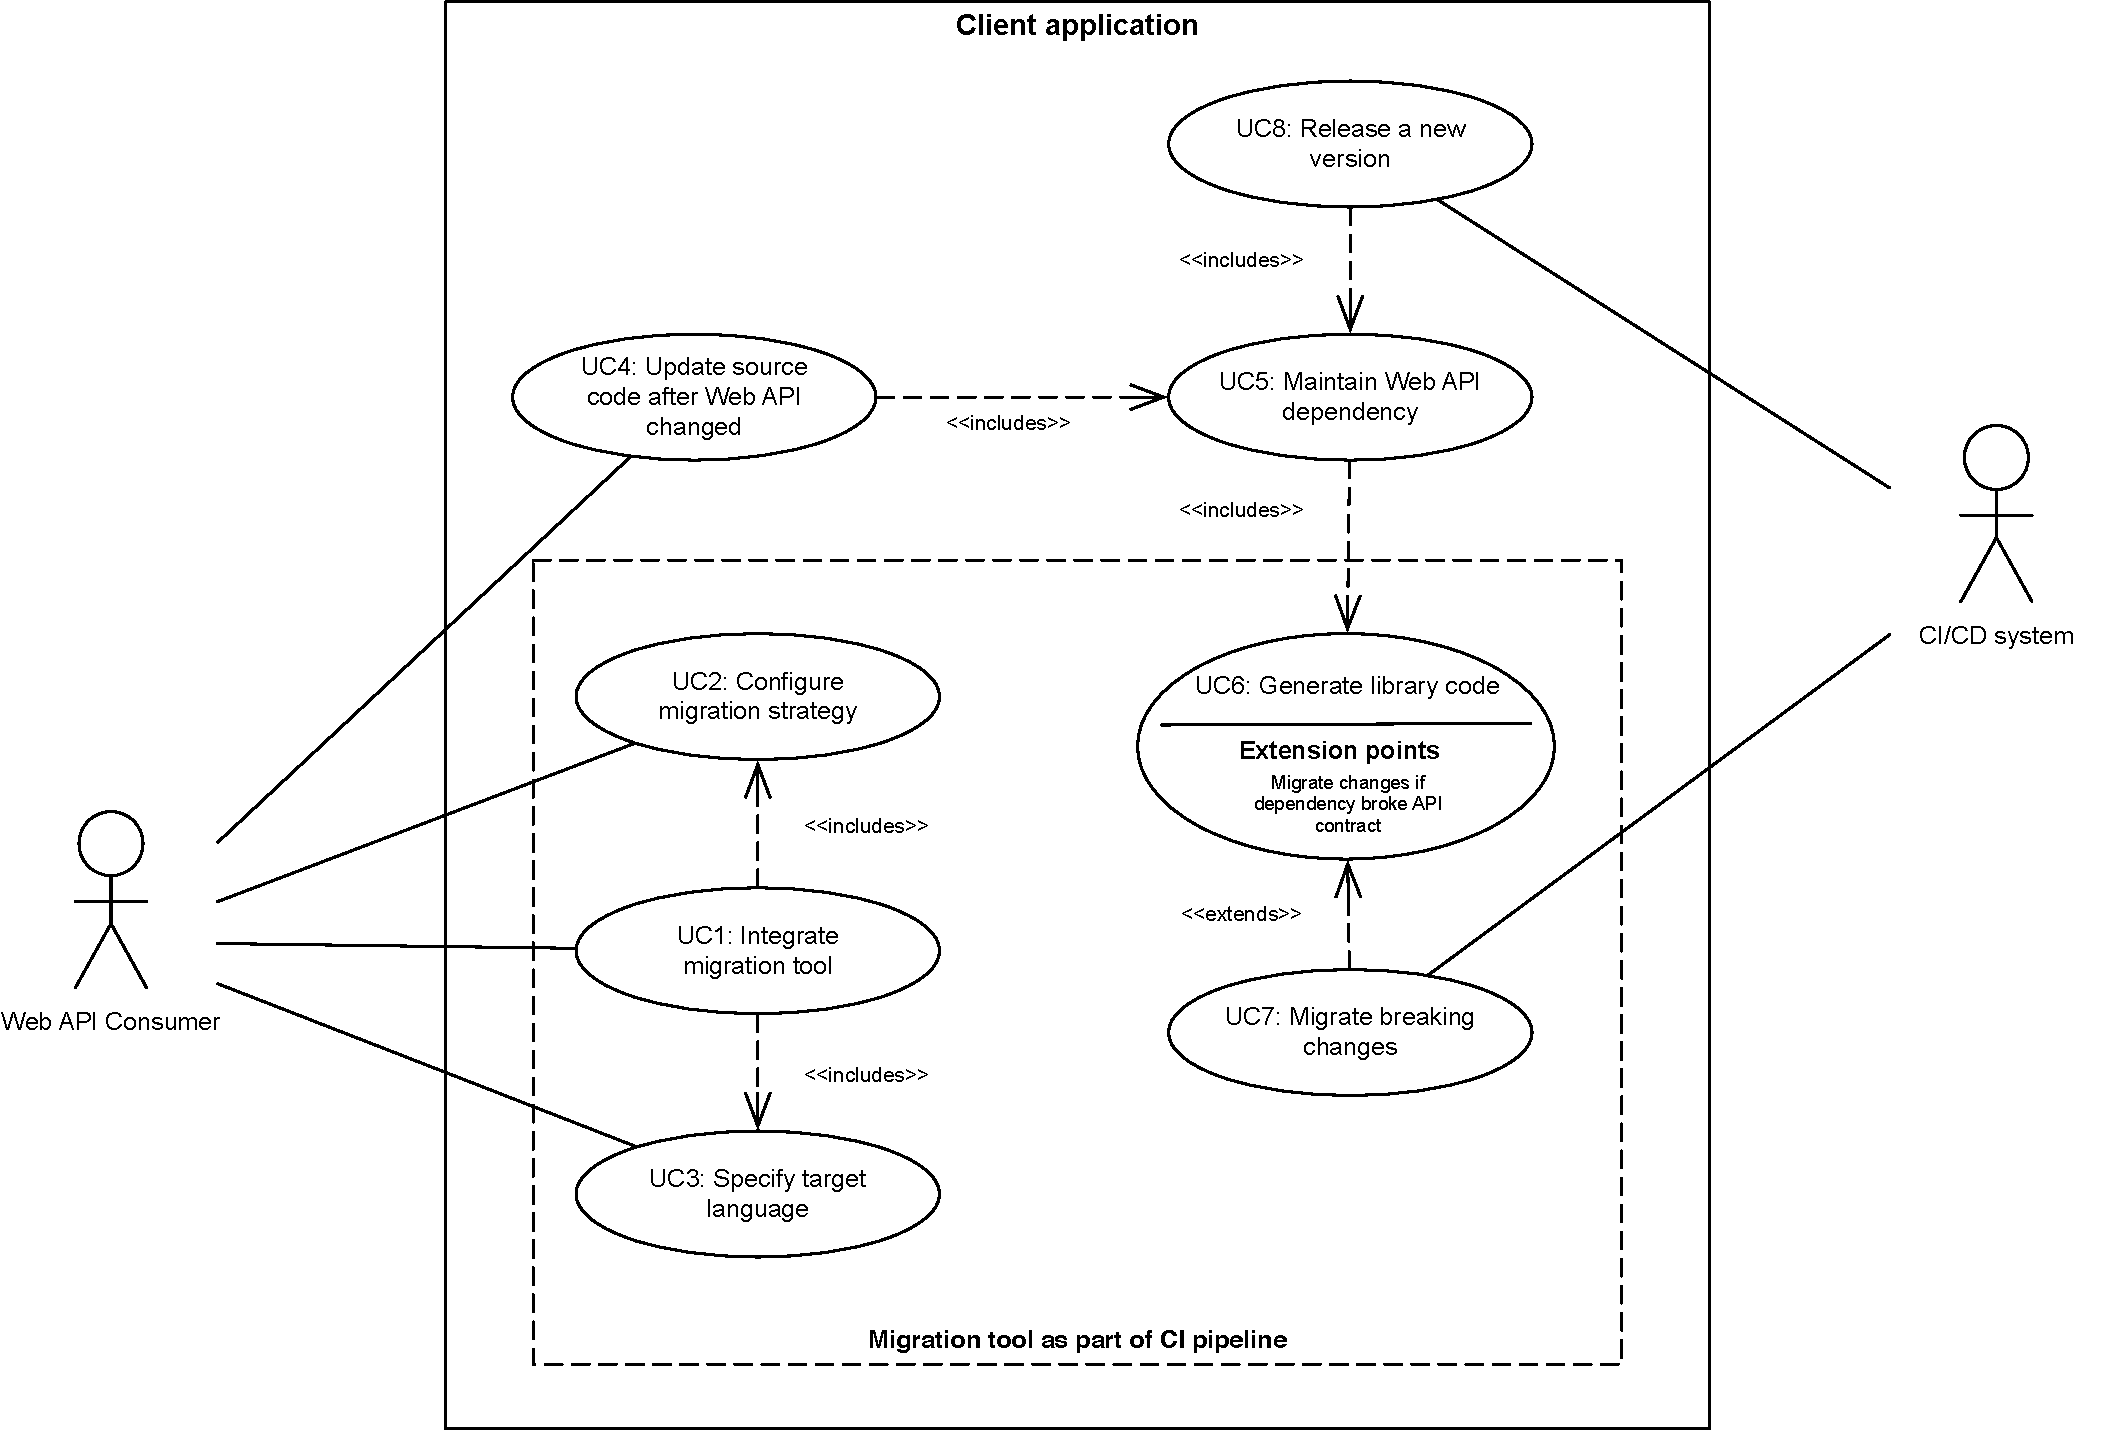
\includegraphics[width=155mm]{images/usecase_consumer.pdf}
		\caption{Use cases of Web API consumers}
		\label{fig:useCaseConsumer}
	}
\end{figure}

The migration tool is modeled as a subsystem of the client application due to its integration into the application's CI/CD pipeline. Integrating the tool requires Web API consumers to specify the target programming language for the generated library code. Furthermore, a migration strategy can be configured to meet the specific needs of the client project. Although both activities are part of the integration use case, they are modeled explicitly for client projects that do not use a CI/CD pipeline. 

Updating source code after a Web API dependency changed is the most important use case for Web API consumers. In addition to generating library code from a Web API's IDL document, our system migrates all changes as stated in its migration guide. This migration guide is created and published by Web API providers. The corresponding use case (\texttt{UC11}) is shown in figure \ref{fig:useCaseProvider}. 

The CI/CD system is modeled as a separate actor to illustrate the use cases that do not require manual interaction by client developers. Its primary task is to create a release of a new version of the client application without breaking changes that were introduced in the Web API. Therefore, it automatically migrates all of these changes by using our system.

For further explanation, the two most important use cases for Web API consumers are described in detail below.
\newpage
\subsubsection{Integrate Migration Tool}
\label{subsubsec:UseCase:IntegrateTool}

\vspace{-2mm}
\begin{center}
    \def\arraystretch{1.5}
    \begin{longtable}{ p{0.22\linewidth} p{0.72\linewidth} }
    \hline
        \textit{Source} & Web API consumer\\
    \hline
        \textit{Stimulus} & Client application needs to incorporate and persist a Web API. \\
    \hline
    	\textit{Environment} & \textbf{Preconditions:} The client application uses a CI / CD pipeline into which the migration tool can be integrated. The interface of the desired Web API is described using an IDL document.
    	
    	\textbf{Postcondition:} The resulting library must be added as a dependency to the client application.
    	\\
    \hline
    	\textit{Artefact} & Migration tool\\
    \hline
    \textit{Response} &
    \vspace{-5.1mm}
    \begin{enumerate}[itemindent=-9pt, leftmargin=14pt, itemsep=0pt, align=left]
    	\item The migration tool gets integrated as part of the CI/CD pipeline of the client application. Therefore, its configuration is either provided as a file via URI or via \ac{CLI} parameters. Optionally, a code formatting ruleset can be specified via its configuration file URI.
        \item The migration tool retrieves the IDL document from its URI.
        \item The migration tool parses the information from the IDL document and generates library code encapsulating lower level HTTP calls. This code is for internal use only and cannot be accessed publicly.
        \item The migration tool generates a public facade layer to persist the current view on the Web API by abstracting calls to the previously generated library code. 
        \item The migration tool generates related meta files to facilitate integrating the output via dependency management.
    \end{enumerate} \\ [-5mm]
    \hline
    \textit{Response Measure} &
    \vspace{-8.5mm}
    \begin{itemize}[itemindent=-9pt, leftmargin=14pt, itemsep=0pt, align=left]
       	\item Error: Execution fails if the IDL document is unavailable or incorrect.
       	\item Success: Output compiles and requests/responses to/from the Web API are processed without errors. 
        \vspace{-5mm}
    \end{itemize}\\
    \hline
    \end{longtable}
\end{center}
\newpage
\subsubsection{Update Source Code After Service Change}
\label{subsubsec:UseCase:FixClientApp}

\vspace{-2mm}
\begin{center}
    \def\arraystretch{1.5}
    \begin{longtable}{ p{0.22\linewidth} p{0.72\linewidth} }
    \hline
        \textit{Source} & Web API consumer\\
    \hline
        \textit{Stimulus} & The client application crashes after a modified Web API is published.\\
    \hline
    	\textit{Environment} & \textbf{Preconditions:} 
    	\begin{itemize}
    		\item The client application integrates a Web API via library code generated by our migration tool. 
    		\item Execution is either triggered manually or as part of a CI/CD pipeline of the client application. 
    		\item The latest release of a Web API introduced breaking changes either to its public interface or behavior. 
    		\item The Web API provider published a machine-readable migration guide along with an updated IDL document.
    	\end{itemize}
    	
    	\textbf{Postcondition:} Client application's dependency must be updated to use the latest version of the generated library code.
    	\\
    \hline
    	\textit{Artefact} & Migration tool\\
    \hline
    \textit{Response} &
    \vspace{-5.1mm}
    \begin{enumerate}[itemindent=-9pt, leftmargin=14pt, itemsep=0pt, align=left]
        \item The migration tool retrieves the updated IDL document and the migration guide from their URIs.
        \item The migration tool checks the changes specified in the migration guide for consistency and correctness. If this check fails, execution is aborted and an error is raised.
        \item The migration tool parses the information from the IDL document and generates library code encapsulating lower level HTTP calls. This code is for internal use only and cannot be accessed publicly.
        \item The migration tool uses the information from the migration guide to adapt the behavior of the previously generated facade layer without modifying the public interface of the facade.
        \item The migration tool generates related meta files to facilitate integrating the output via dependency management.
    \end{enumerate} \\ [-5mm]
    \hline
    \textit{Response Measure} &
    \vspace{-8.5mm}
    \begin{itemize}[itemindent=-9pt, leftmargin=14pt, itemsep=0pt, align=left]
    	\item Error: Execution fails if the IDL document is unavailable or incorrect.
       	\item Error: Execution fails if changes stated in the migration guide are contradicting or incompatible.
       	\item Success: Output compiles and requests/responses to/from the Web API are processed without errors. 
        \vspace{-5mm}
    \end{itemize}\\
    \hline
    \end{longtable}
\end{center}

Web API providers are the second group of actors that participate in our proposed workflow. Figure \ref{fig:useCaseProvider} shows the typical use cases of our system from their perspective.

\begin{figure}[h]
	\centering{
		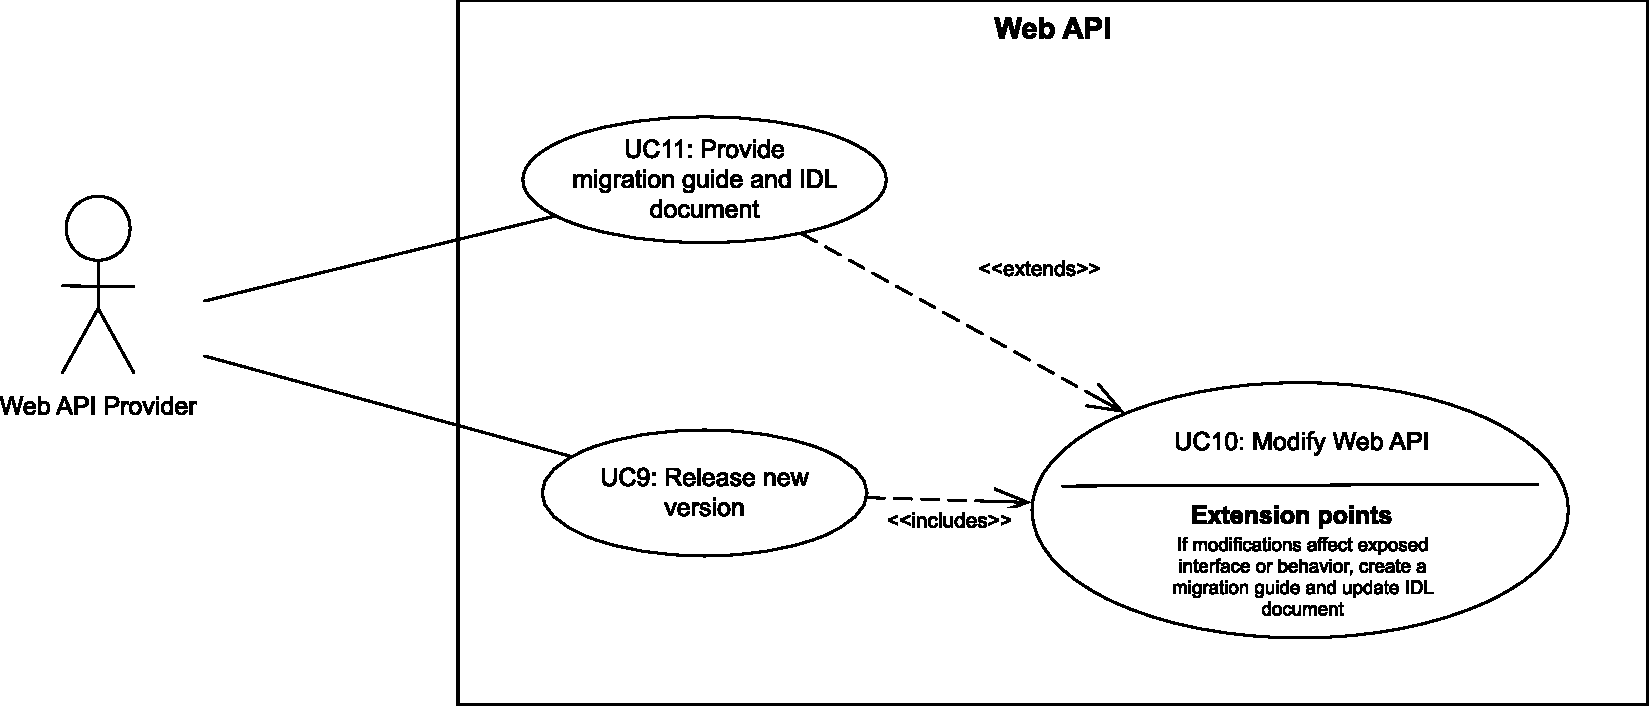
\includegraphics[width=150mm]{images/usecase_provider.pdf}
		\caption{Use cases of Web API providers}
		\label{fig:useCaseProvider}
	}
\end{figure}

Web API providers need to decide whether to introduce breaking changes to the publicly available interface or behavior. When breaking changes cannot be avoided, providers must create a machine-readable migration guide that specifies them. Furthermore, they need to provide an updated IDL document describing the current state of the Web API. Since our proposed workflow is only slightly different from their current workflow, a detailed description of a provider's use case focuses on providing a migration guide and an IDL document.

\subsubsection{Provide Migration Guide and IDL document}
\label{subsubsec:UseCase:MigGuideIDL}

\vspace{-2mm}
\begin{center}
    \def\arraystretch{1.5}
    \begin{longtable}{ p{0.22\linewidth} p{0.72\linewidth} }
    \hline
        \textit{Source} & Web API provider\\
    \hline
        \textit{Stimulus} & New functionality was added to the Web API or existing behavior was changed. Therefore, a new version of the Web API is released. \\
    \hline
    	\textit{Environment} & \textbf{Preconditions:} The provider introduced breaking changes to the exposed interface or behavior when modifying the Web API.
    	
    	\textbf{Postcondition:} The output needs to be published on a publicly accessible server and its URI has to be provided to Web API consumers.
    	\\
    \hline
    	\textit{Artefact} & Migration guide, IDL document\\
    \hline
    \textit{Response} &
    \vspace{-5.1mm}
    \begin{enumerate}[itemindent=-9pt, leftmargin=14pt, itemsep=0pt, align=left]
    	\item The IDL document must describe the publicly exposed interface and behavior. The Web API provider can either manually create this document or generate it using tools.
    	\item The migration guide must contain the type of IDL used to describe the Web API.
    	\item The migration guide must contain the type of Web API.
    	\item The migration guide must contain both the previous and the current version number according to the semantic versioning principles.
    	\item The migration guide can contain a short textual summary to provide an overview of the changes introduced in the current version.
    	\item The migration guide must contain a list of all breaking changes introduced in the current version. 
    \end{enumerate} \\ [-5mm]
    \hline
    \textit{Response Measure} &
    \vspace{-8.5mm}
    \begin{itemize}[itemindent=-9pt, leftmargin=14pt, itemsep=0pt, align=left]
       	\item Success: The migration guide can be retrieved and parsed by migration tool.
       	\item Success: The IDL document can be retrieved and parsed by migration tool.
        \vspace{-5mm}
    \end{itemize}\\
    \hline
    \end{longtable}
\end{center}

Currently, Web API providers have to manually create a migration guide. We propose that future research should explore automating this task to reduce the effort for providers. Existing tools for automatic generation of IDL documents can serve as a reference here.